\chapter{GPS Concept and Error Sources}\label{ch:GPS_concept}

Along with earlier navigation systems, this chapter explains the positioning concept of GPS and modern Global Navigation Satellite Systems in general.
The error sources that impact the accuracy of GPS are listed and split into categories that determine in which segment those errors occur.


\section{Predecessors}
Before there was GPS, other radionavigation systems were used.
They were mostly ground based and limited to a certan area or time.

One of the early examples is the U.S. system \textit{Loran}.
It works with multiple transmission stations with a distance of about 1000km to each other.
They send out pulse signals in all directions.
With the difference in time-of-arrival of those pulses, a receiver can triangulate its position.
This method is one variant of hyperbolic positioning.
Only a 2D fix can be acieved with such systems.
The height, if needed, has so be determined with a different method.
The development of \textit{Loran-A} was started during World War \rom{2}.
\textit{Loran-C} is the latest version and still in use today
It has a rms positioning accuracy of about 250m.

Another hyperpolic positioning system was \textit{Omega}.
It was the first global radionavigation system and operational from 1970 to 1997.
But rather than measuring the time differene of pulses, the phase difference of sinusoidal signals was measured.
This method resulted in a rms postitoning accuracy of 2-4km.
The lower accuracy can be explained with the much wider area it had to cover.

Apart from those ground based systems, there was a working satellite navigation system that came even before \textit{Omega}.
It is called \textit{Transit} and was operational from 1964 to 1996.
A doppler based systen that was launched by the U.S. Navy.
In doppler positioning, a 2D position can be determined from the time the doppler of the satellite signal changes from high to low and the sharpnes of the change.
At the moment the doppler changes, the satellite is the closest to the receiver on its orbit.
The distance from the projected orbit can then be determined by how sharp the doppler changes.
When the receiver is directly on the projected orbit, the doppler changes the fastest.
In contrast to modern GNSS, \textit{Transit} satellites had polar orbits with a low altitude of 1100km.
Only one satellite was visible at a time with a wait time of up to 100 minutes between them.
This made positioning a relatively long process, but the rms positioning accuracy was much better with 25m.

A range of counterparts from Russia and Eurpoe existed to those U.S. systems.
\textit{Gee} was a hyperbolic system from Great Britain similar to Loran.
It was used by the Royal Air Force during World War \rom{2}.
Doppler positioning was already used in reverse to determine the orbit of \textit{Sputnik \rom{1}} from a ground station with a known location.
The idea to measure the postiton on earth came from this application.
The Soviet Union had two dopple based system similar to \textit{Transit} called \textit{Parus} and \textit{Tsikada}. \cite{misra2011global}


\section{Global Navigation Satellite Systems}

From the knowledege gained from \textit{Tansit}, a new class of space based navigation systems emerged. 
The first one beeing the NAVSTAR Global Positioning System (GPS) developed by the U.S. Government.
The first GPS satellite was launched in 1978 and the system became fully operantional in 1993.
To be independent from the U.S. when it comes to navigation and improve local positioning, other nations started to launch their own systems.
The generic term for such systems is Global Navigation Satellite Systems (GNSS).
The fisrt addition to the group was the former Soviet and now Russian system GLONASS.
It is very similar to GPS in terms of use case and architecture.
Both were mainly developed for military use and designed to cover the whole globe with a full constellation of 24 satellites in medium earth orbit. \cite{misra2011global}

A newer addition is the european system GALILEO.
It is similar in terms of system architecture to GPS and GLONASS, but it is the first GNSS that is under civilian controll.
This guarantees that civil receivers can get the highest precission possible.
The GALILEO constellation is not yet complete with 14 usable satellites at the moment, but it is said to improve the accuracy to the centimeter level in normal operation. \cite{GSA_Galileo}

Beside global navigation systems, there are also local programs which improve the regional accuracy.
They consist of satellites in geostationary or geosynchronous orbits.
This gives them a constant location above the earth or within a few degreees of longitude.
Such systems are the Japanese QZSS and the Indian IRNSS.
The Chinese BeiDou system is a combination of global and regional.
It started with just geostationary and geosynchronous satellites over China, but now has three operational global satellites with more to come.


\section{GPS}

This section closer explains the system architecture, functional principle and performance of GPS.
The difference to the ohter GNSS is minor.
Orbits, frequencys and signal modulation are slightly different between the systems, but the basic architecture is the same.


\section{System Architecture}

The GPS system can be split into three segments.
The Space Segment includes the satellites, the Control Segment is the ground equipment that manages the satellites and the User Segment are the receivers.

\subsubsection{Space Segment}

A full GPS constellation consists of 24 satellites as shown in figure \ref{fig:constellation}.
Currently, there are 31 GPS satellites in operation.
They are in medium earth orbit at an altitude of about 20'200km with each satellite circling the earth twice a day.
About 8 satellites are visible to a user at a time.
These satellites are constantly beeing replaced by newer ones with new features.
The different generations of satellites are divided into Blocks.
Starting with the first generation of satellites launched from 1978 until 1995 called Block \rom{1}.
Block \rom{2} satellites had a series of incremental improvements and added new signals over the time they were launced from 1989 until 2016.
The separate satellite series of the Block \rom{2} generation were called II, IIA, IIR, IIR-M and IIF.
The first Block \rom{3} launch is scheduled for 2018.
The third generation adds even more signals and trinsmitts at higher power levels.

\begin{figure}[ht]
 \centering
 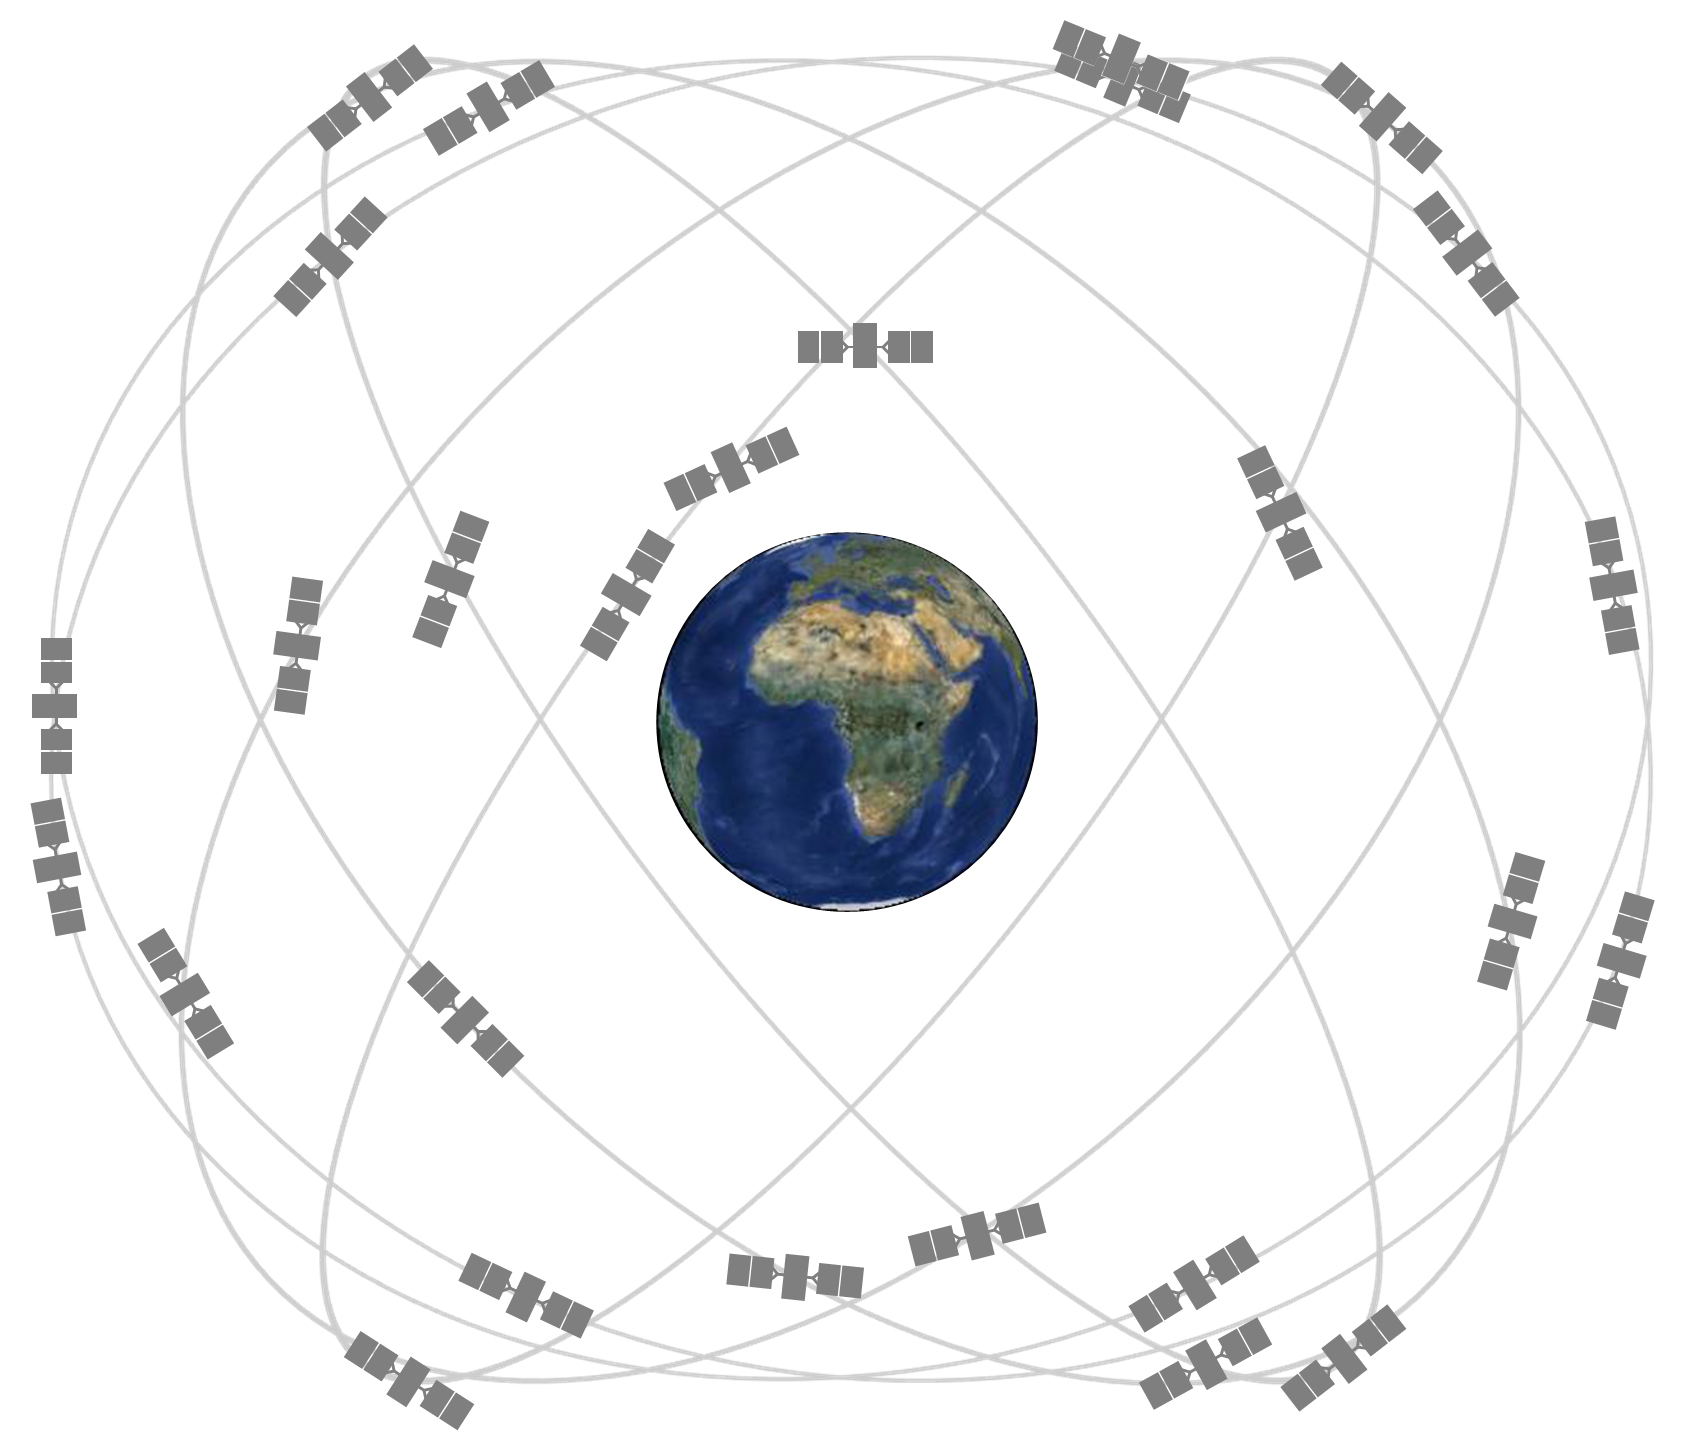
\includegraphics[height=5cm]{images/constellation.jpg}
 \caption{GPS satellite constellation \cite{GPS_GOV}}
 \label{fig:constellation}
\end{figure}

\subsubsection{Control Segment}

To ensure an accurate positioning service for GPS users, the satellites have to be constantely monitored and maintained.
This is the job of the Control Segment.
It monitors satellite orbits and time to predict satellite ephemerides and clock parameters.
It then updates the satellite navigation data, which is later sent from the satellite to the user.
If neccesary, the Control Segment can order the satellites to performe maneuvers to maintain a correct orbit or to relocate to another orbit.
The Control Segment comprises of a network of ground based stations spread arround the globe.
This network is coordinated by the Master Controll Station in the U.S. state of Colorado.

\subsubsection{User Segment}

Finally, the User Segment is where the satellite signals are picked up and the position of the user is calcuated.
Unlike the other segments, the User Segment is not developed by the U.S. Government, apart from military receivers.
The design of civil GPS receivers is left to market forces.
The size of those receivers droped dramatically during the lifetime of GPS from the size of a backpack, to the size of a single microchip.


\subsection{Functional Principle}

GPS works with the principle of trilateration.
For this method of postitoning, the distance to three known lacations is needed to calculate the own position in three dimensions.
This works with basic vector geometry.
The euclidean distance between two points in three-dimensional space can be calculated with equation \ref{eq:euclidean_dist}.

\begin{equation}
 r^{(k)} = \sqrt{(x^{(k)} - x)^2 + (y^{(k)} - y)^2 + (z^{(k)} - z)^2} = \lvert\lvert \textbf{x}^{(k)} - \textbf{x} \rvert\rvert		\label{eq:euclidean_dist}
\end{equation}

For GPS, the two points are the user position $[x, y, z]$ and the satellite position $[x^{(k)}, y^{(k)}, z^{(k)}]$ and the true distance between them is called $r^{(k)}$.
The satellites are distinguished with the superscript $^{(k)}$ where k stands for the k-th satellite in view.
In theory, with the position and distance of three satellites, a system of equations could be constructed and the three variables of the user position $[x, y, z]$ could be estimated.
But in practice, a gps receiver needs at least four satellites to estimate its position.
This is because a fourth variable needs to be estimated called $\delta t_u$.
This is the difference between GPS time and user time.

\begin{figure}[ht]
 \centering
 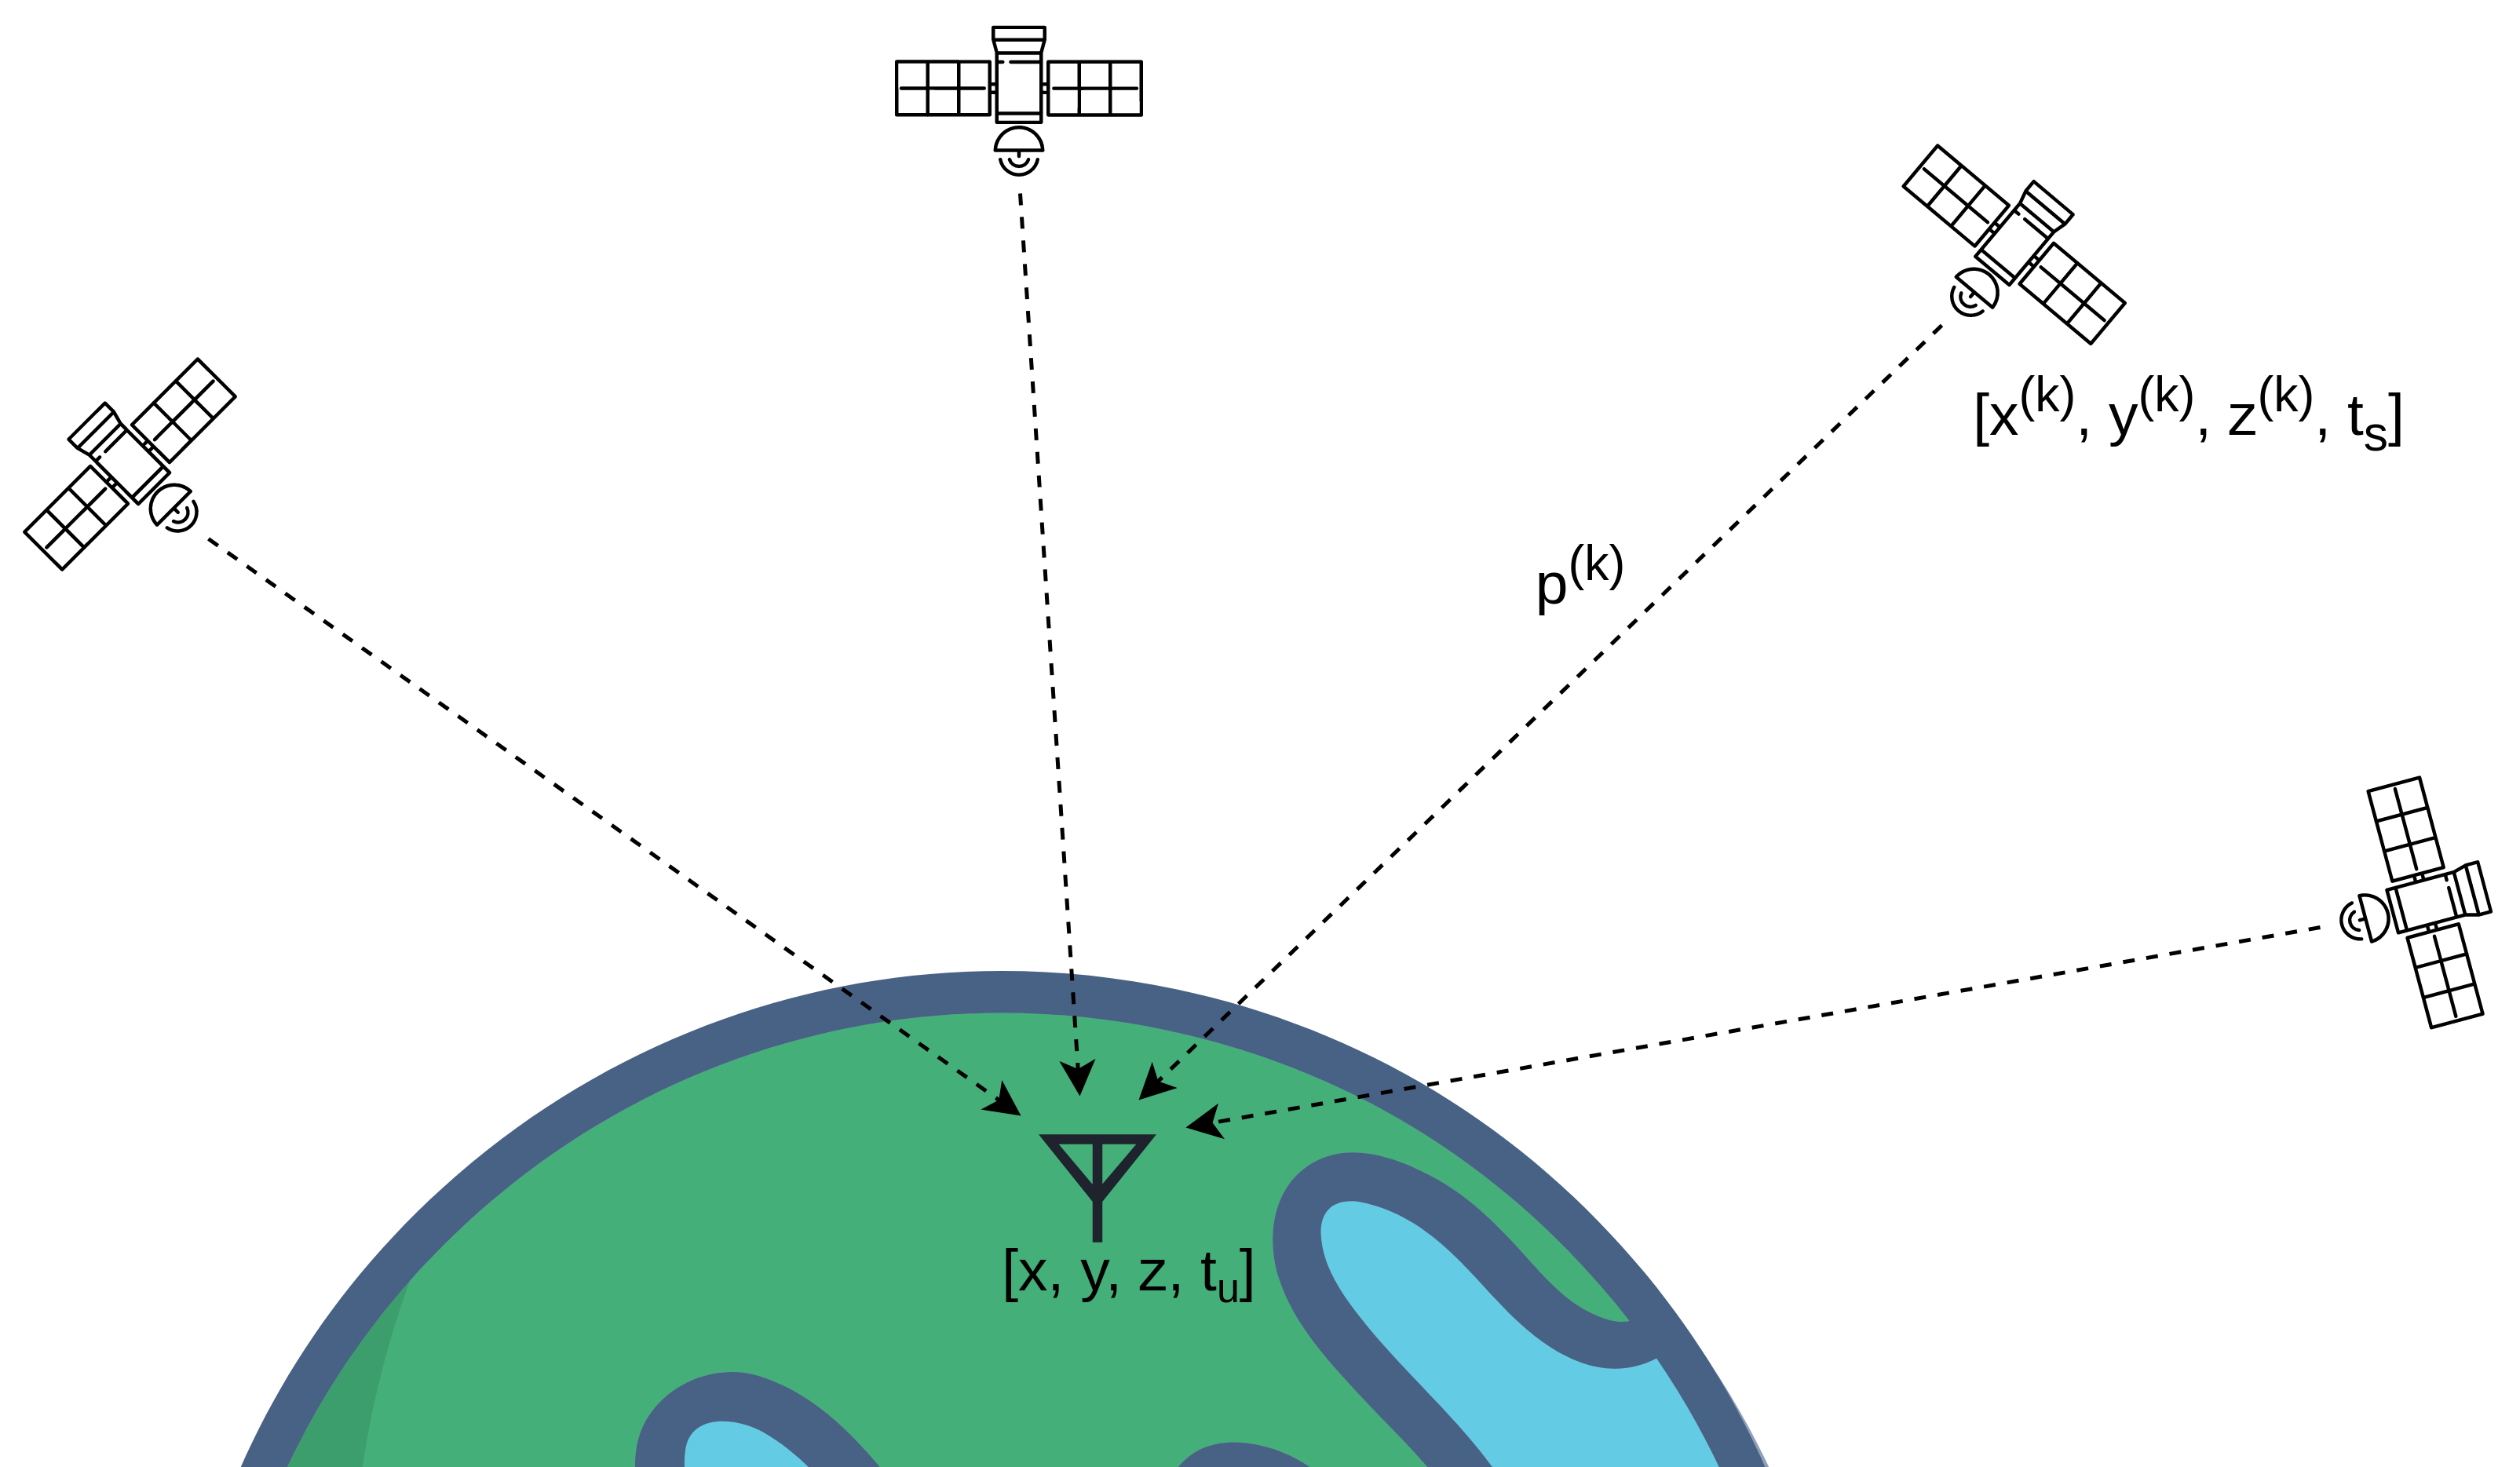
\includegraphics[width=0.8\textwidth]{images/Position_Estimation.png}
 \caption{GPS triangulation}
 \label{fig:triangulation}
\end{figure}

GPS uses the propagation time of radio waves to determine the distance between satellite and user.
The measured transmision time is multiplied by the speed of light to get the distance in meters.
This is not the true distance $r^{(k)}$.
Insted, the so called pseudorange $\rho^{(k)}$ is measured, which contains the true range and a set of errors.
The relation is shown in equation \ref{eq:pseudorange}.
The pseudorange contains the clock errors $c[\delta t_u - \delta t^{(k)}]$ and the atmospheric errors $I^{(k)} + T^{(k)}$.
Those errors can be modeled and estimated to correct the pseudorange.
All the errors that can not be modeled are combined in the term $\varepsilon^{(k)}$.
What they mean is closer explained in section \ref{sec:error_sources}.

\begin{equation}
 \rho^{(k)} = r^{(k)} + c[\delta t_u - \delta t^{(k)}] + I^{(k)} + T^{(k)} + \varepsilon^{(k)}		\label{eq:pseudorange}
\end{equation}

Important here is the user clock error $\delta t_u$.
The reason for this error is the unprecise clock in the receiver.
The satellites have atomic clocks which are synchorinized to GPS time.
It is not feasable to build an atomic clocks into every receiver and keep it synchorinized to GPS time.
Insted, the difference between receiver time and GPS time is estimatet with the measurement from a fourth satellite.
This is possible because the user clock error is common in the pseudoranges from all satellites.
The estimation of the four variables $[x, y, z, \delta t_u]$ is either done iteratively with the Least Square method or with a Kalman Filter.

\subsection{Signals}

A GPS receiver can work with only the information included in the signals from the satellites.
This means the information for distance and satellite position have to be transmitted with those signals.
GPS solves this problem with a three-layered signals like the one in figure \ref{fig:signal_structure}.

\begin{figure}[ht]
 \centering
 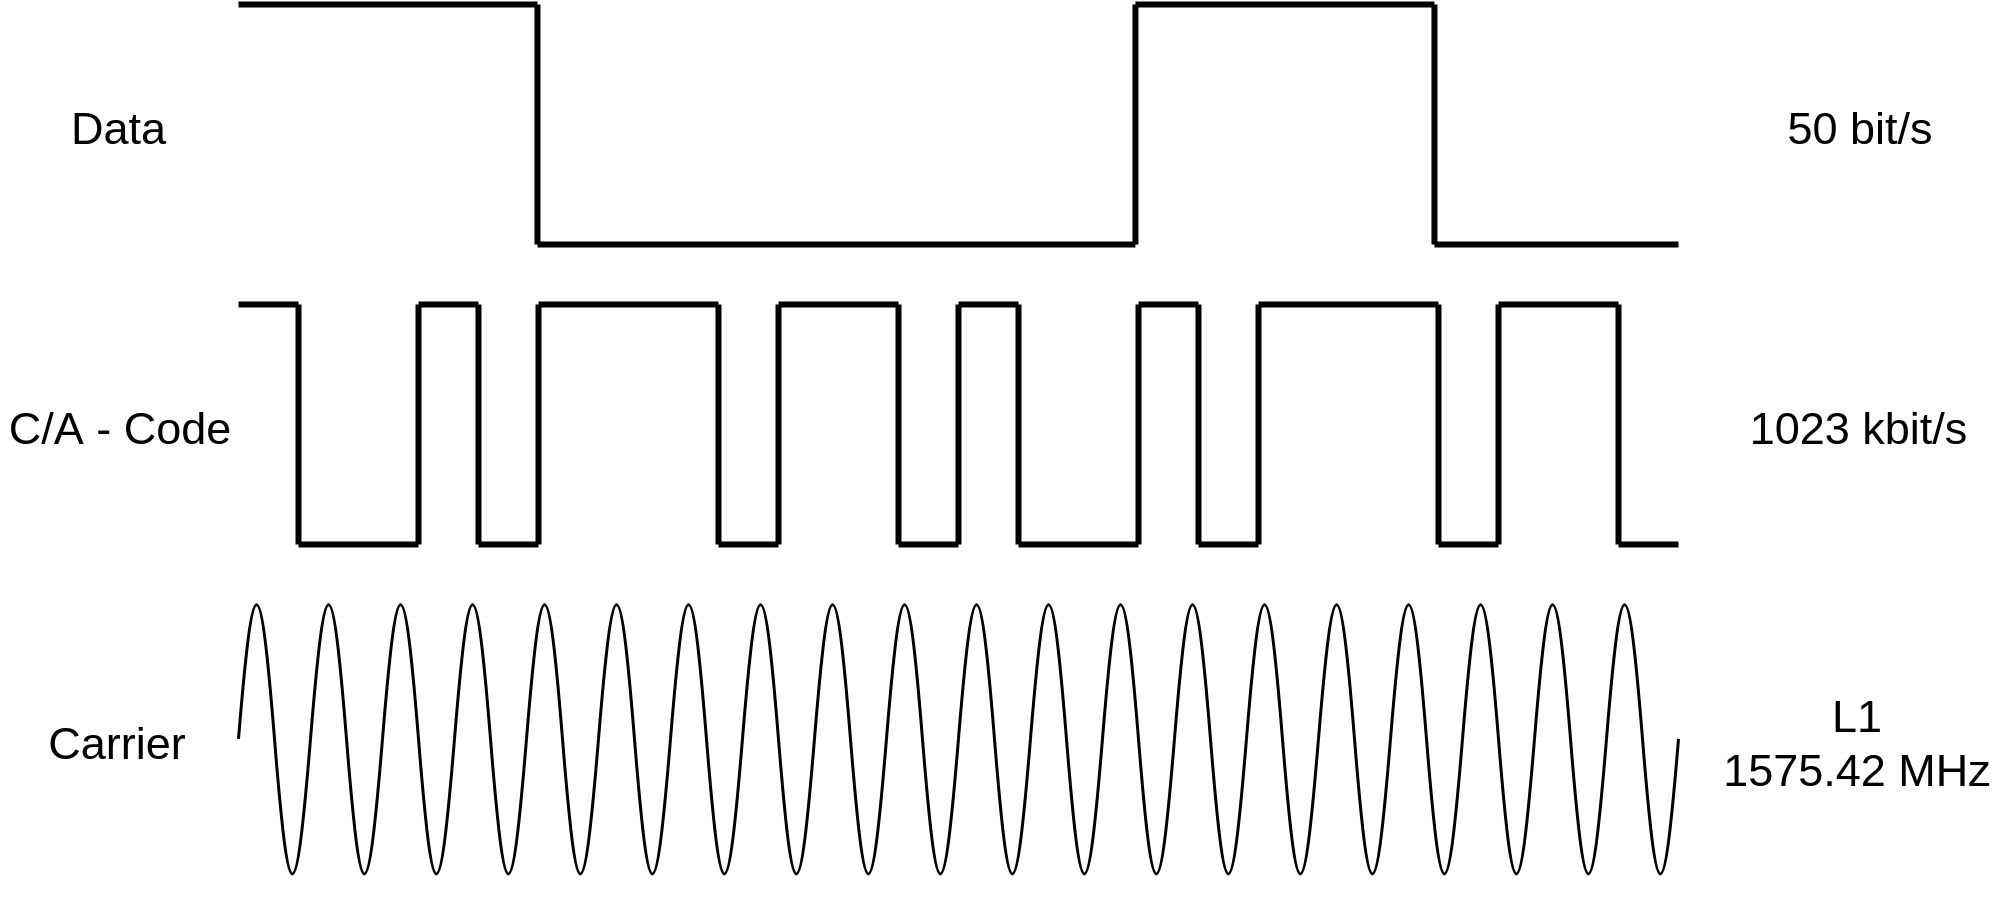
\includegraphics[width=0.8\textwidth]{images/Signal_Structure.png}
 \caption{C/A-code signal structure (not to scale)}
 \label{fig:signal_structure}
\end{figure}

The carrier is a sinusoidal signal in the L band.
Most civil GPS receivers work with the L1 signal at 1575.42MHz.
GPS satellites also send on L2 at 1227.6 MHz and newer satellites on L5 at 1176.45 MHz too.
A variety of civil and encrypted military signals are modulated onto those carriers.
The main signal for civil applications is the C/A-code on L1.
It consists of the C/A-code itself and a data stream.
The C/A-code and the data stream are both binary sequences.
They are first XORed together and then modulated onto the carrier using \textit{binary phase shift keying} (BPSK).
This process of XORing is equal to the spreading of the spectrum with the pseudorandom C/A-code sequence.

The C/A-code is a sequence of 1023 bits, which repeats every millisecond and is unique to each satellite.
The lenght of each bit, or chip in this context, is about $1\mu s$.
Besides the spreading and despreading of the spectrum, this code is used to measure the signal transmission time.
The received signal is demodulated and correlated with local copies of the C/A-codes on separate channels.
The local copy is shifted in time until an autocorrelation peak emerges.

The actual data transmitted with only 50bit/s is the navigation message.
It contains information about the satellites GPS time, orbit, clock correction and ionospheric correction.
The obit data is called ephemeris.
With it, the position of the satellite can be calculated.
The satellites clock and ionospheric corrections are used to correct the pseudorange for the terms $\delta t^{(k)}$ and $I^{(k)}$.

The transmitted GPS time with the current bit location in the navigation message frame and the delay from the code correlation combined make up the pseudorange measurement.

\subsection{Performance}

To evaluate the performance of GPS, a number of metrics can be used.
The most prominent one is of course the accuracy.
This was already addressed in \ref{sec:requirements}, where the requirements were defined.
Accuracy can be explained with the two errors variance and bias.
In GPS, the two errors are often not given separately when the accuracy of the whole system is described.
Accuracy simply describes how close the measurement matches the real position.
The two most used metrics to described GPS postitoning accuracy are the 95th precentile and the root-mean-square error (RMSE).
The 95th precentile describes the border in meters, where 95\% of errors are smaller and 5\% are larger.
The RMSE equals the variance of $1\sigma$, as long as the mean error is zero.
A mean error is a bias, that is considered in the RMSE but does not impact the variance.
RMSE is calculated with:
\begin{equation}
 RMSE = \sqrt{\frac{\sum\limits_{i=1}^n \lvert\lvert \textbf{x}_{real} - \textbf{x}_{meas} \rvert\rvert^2}{n}}
\end{equation}

Accuracy can be further divided into horizontal and vertical error.
The GPS SPS(Standard Positioning Service) Performance Standard defines an average $\leq$9m 95\% horizontal error and a $\leq$15m 95\% vertical error \cite{SPS_Performance}.

Other than accuracy, availability and integrity are two other important metrics.
The availability is the likelihood a user anywhere on earth can get a GPS fix.
The GPS SPS Performance Standard defines an average $\geq$99\% locational availability \cite{SPS_Performance}.
Integrity is how trustworthy the information of the system is.
This is especially important for safety-of-life applications like airplane navigation.
GPS constantly monitors itself and informs the user if the data does not meet the requirements.
This is done with satellite self-monitoring, cross-monitoring between satellites, and ground based monitoring.


\section{Error Sources}\label{sec:error_sources}

The error in the GPS position is determined by two Factors.
The reason there is a position error at all are the errors in the measured distances to the satellites called User Range Error (URE).
These errors are further divided into three groups depending on where they occure.
Errors in the parameters broadcasted by the satellites are here called satellite errors.
Errors that occure in the signal path from the satellite to the receiver are called atmospheric errors.
Finally, errors that are caused by unprecise measurenents of the signals by the receiver are called measurement errors.
All three types are discussed later in this section.

The other factor is the satellite geometry.
It determines how much the URE impacts the position accuracy.
An optimal geometry would be stellites evenly distributed in all three dimensions.
This is not possible because a receiver on the surface of the earth can not receive signals from satellites blocked by the earth.
A metric to determine the geometry quality is the Dilution of Precision (DOP).
Different versions of DOP can be determined like the Horizontal DOP (HDOP), Vertical DOP (VDOP), 3-D Position DOP (PDOP) and Time DOP (TDOP).
The RMS position error can then be calculated with the standard deviation of the URE $\sigma_{URE}$ multiplied with the corresponding DOP.
For example, the horizontal RMS position error can be calcuated with:
\begin{equation}
 RMS \text{(horizontal position error)} = \sigma_{URE} \cdot HDOP
\end{equation}

\subsection{Satellite Errors}

\begin{minipage}{0.6\textwidth}
  GPS satellites broadcast a navigation message with 50bps which includes orbital parameters to calculate their position.
  Orbital parameters of a GPS satellite are called ephemeris. 
  Those parameters are estimated and uploaded to the satellites by the controll segment.
  The difference between the estimated position and the real satellite position is called ephemeris error.
  
  The other satellite error comes from an unprecise satellite clock.
  Although GPS satellites have atomic clocks, they can never be perfectly alligned with GPS time.
  That is why the controll segment also estimates a clock offset for each satellit, which is also broadcasted with the navigation message.
  This correction apperars in the pseudorange equation \ref{eq:pseudorange} as $\delta t^{(k)}$.
  
  The remaining satellite errors after the pseudorange correction are the errors in the ephemeris estimation and satellite clock offset estimation.
  They are determined by how accurate the controll segment can determine the position and time of each satellite.
\end{minipage}
\hfill
\begin{minipage}{0.38\textwidth}
 \flushright
 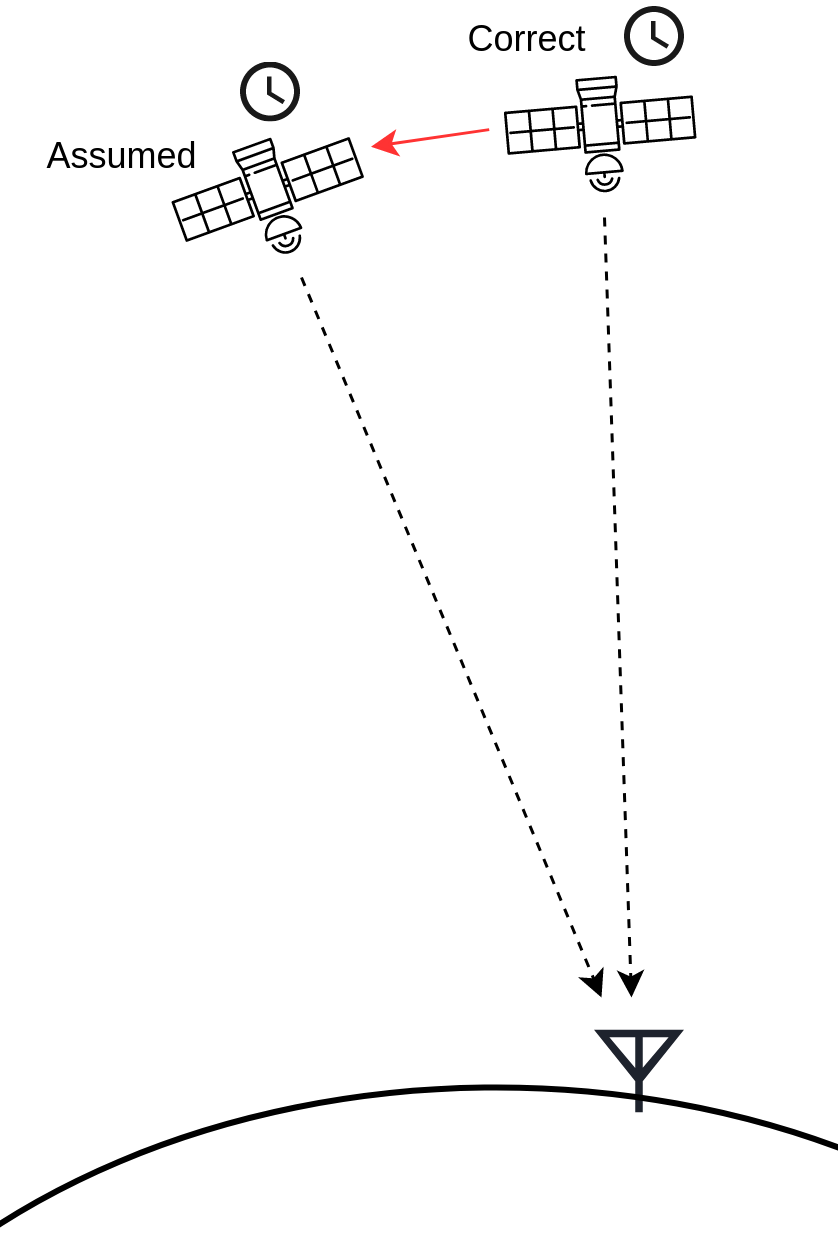
\includegraphics[width=\textwidth]{images/Satellite_Errors.png}
 \captionof{figure}{Ephemeris and time satellite errors}
\end{minipage}

\subsection{Atmospheric Errors}

\begin{minipage}{0.6\textwidth}
  The orbit of GPS satellites is at about 20'000km above the earths surface.
  To measure the pseudorange, the signal transmission time is divided by the speed of light.
  This implies that the signal travels through only vacuum.
  In reality, this is not entirely accurate.
  On the way from the satellite to the receiver, the signal has to pass trough large parts of earths atmosphere.
  Especially two atmospheric layers influence the propagation time of the signal.
  The first one is the ionosphere between about 50km and 1000km.
  It consists of ionized gases.
  The intensity of the ionization depends mainly on the sun's activity and the day/night cycle.
  The ammount of ionization determines the delay added to the transmision time by the ionosphere.
  The zenith delay in meters varies from 1m up to 36m. 
  It can increase by a factor of 3 with a lower elevation of the satellite.
  The ionosphereic delay can be modeled to a certain extent with the current space weather and appers in the pseudorange equation \ref{eq:pseudorange} as $I^{(k)}$.
\end{minipage}
\hfill
\begin{minipage}{0.38\textwidth}
 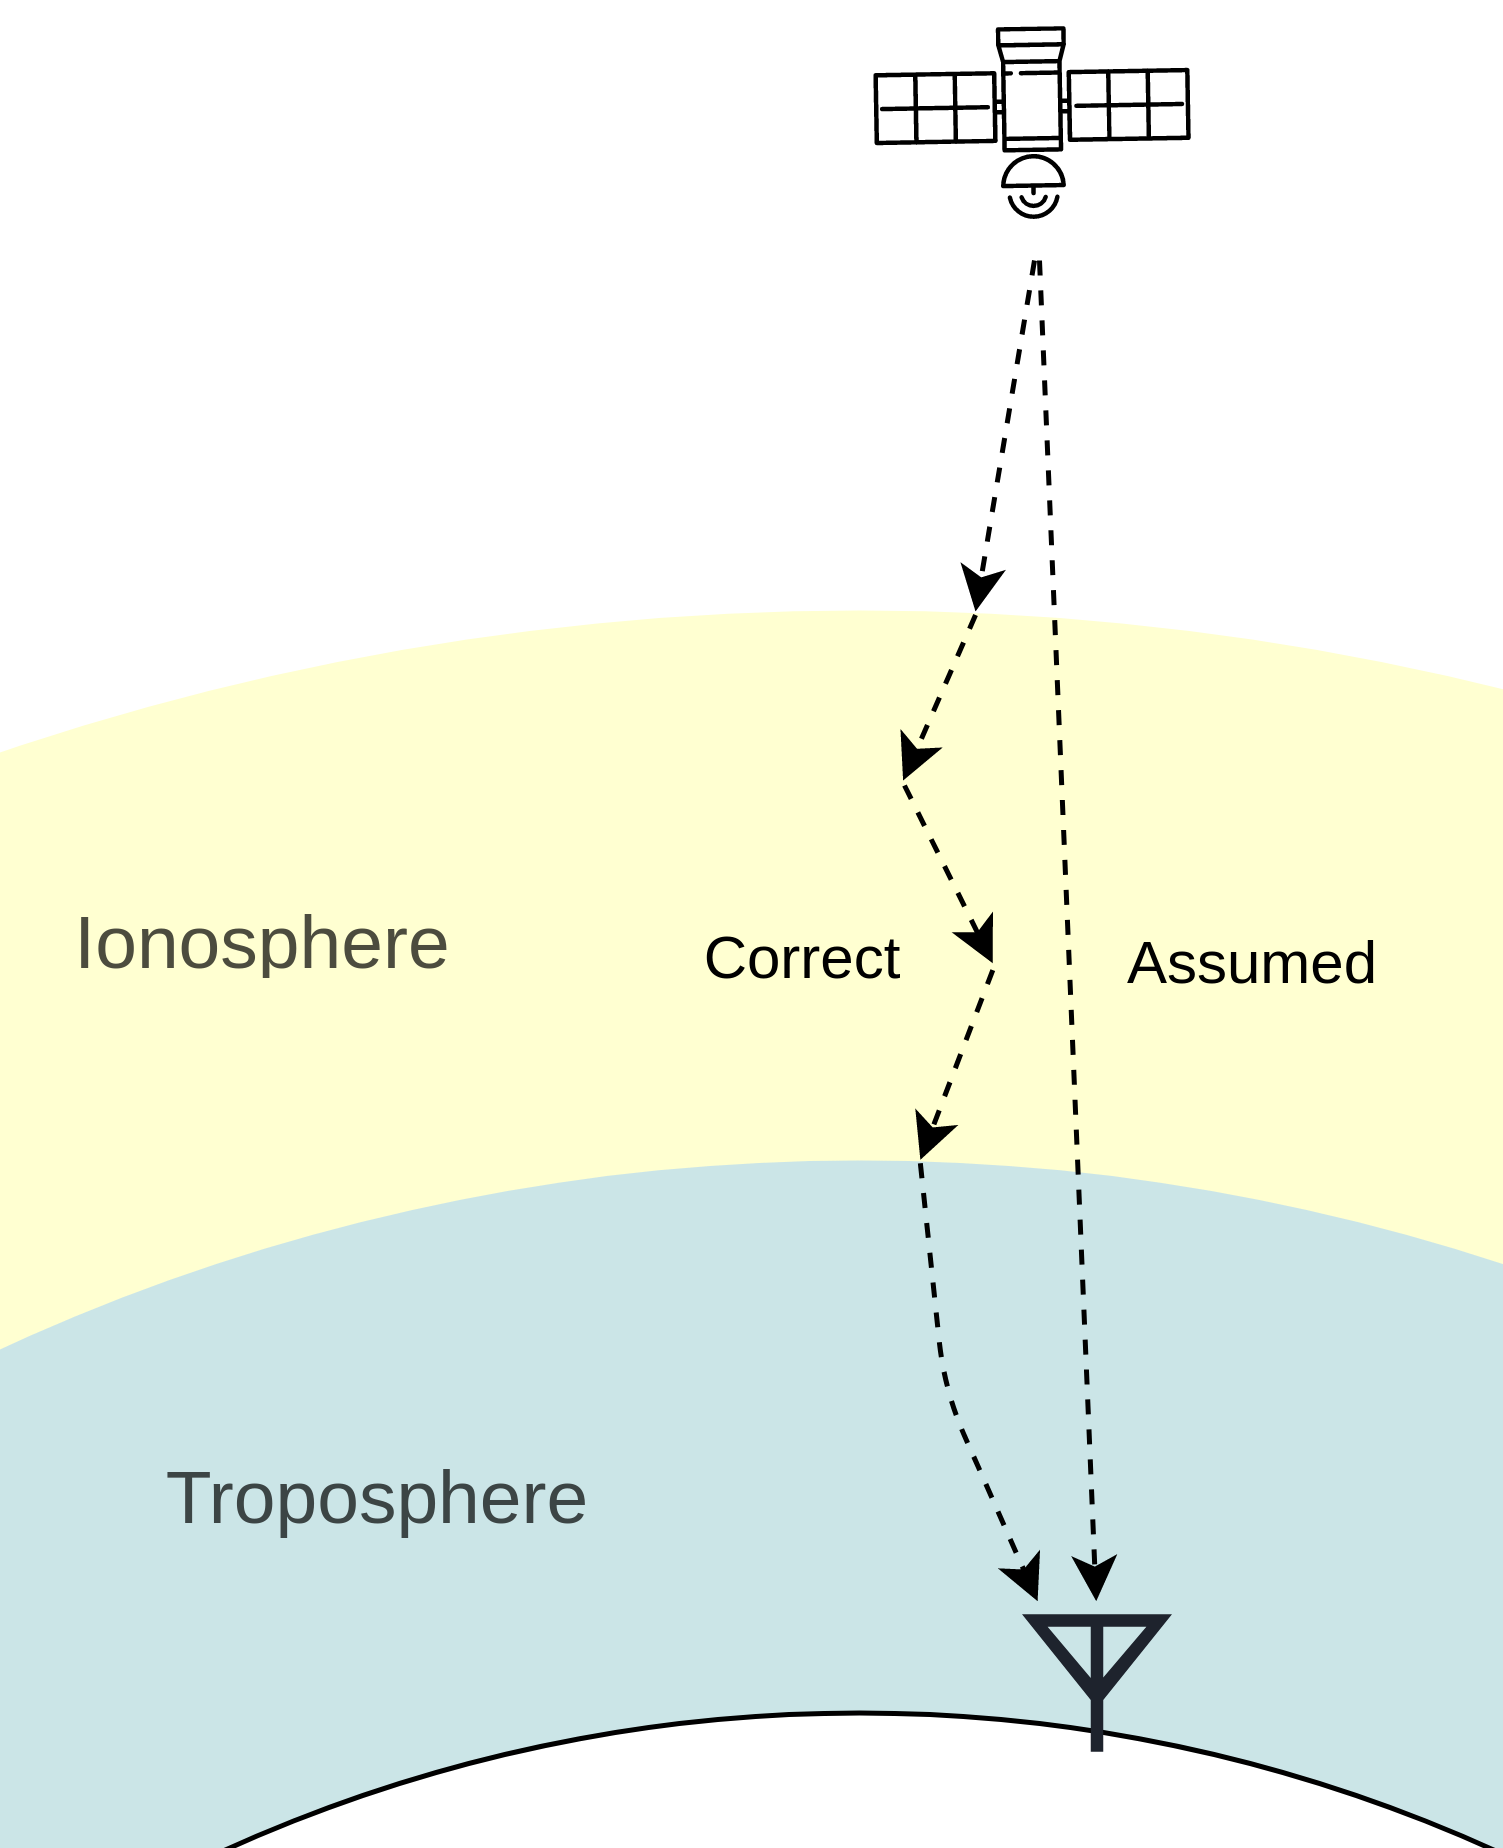
\includegraphics[width=\textwidth]{images/Atmospheric_Errors.png}
 \captionof{figure}{Ionosphereic and tropospheric errors}
\end{minipage}

The other important layer is the troposphere.
It is the lowest part of the atmosphere and extends from the ground to about 9-16km depending on the latitude.
The troposphere contains three-quarters of the gaseous mass and all of the water vapor of the atmosphere.
This matter slows the signal down and results in a zenith delay of 2.3-2.6m at sea level.
With a lower elevation of the satellite, the delay can increas by a factor of 10.
It can be modeled with the atmospheric humidity and pressure, and is fairly stable because the biggest influence has the gaseous mass, which does not change much over time.
The term for tropospheric delay in the pesudorange equation \ref{eq:pseudorange} is $T^{(k)}$.

\subsection{Measurement Errors}

Unlike the previous errors, measurement errors depend on factors like signal power, code structure and receiver design.
Multipath is a problem most wireless communication systems have.
The signal is refelcted by surfaces and arrives at the receiver miltiple times at different times.
Normally, there is a main signal from the line-of-sight path, and weaker delayed versions of the signal.
The influence no the measured range depends on the strength and delay of the reflected signal.

Receiver noise is a general term for noise added by the antenna, amplifiers, cables and the receiver.
It also includes RF radiation noise which is picked up by the antenna.
The strength of the receiver noise relative to the GPS signal determines the signal-to-noise ratio.
A low signal-to-noise ratio results in a tracking error of the GPS code, which in turn directly impacts the pseudorange measurement.

None of those errors can be modeled, so they are included in the term $\varepsilon^{(k)}$ in the pseudorange equation \ref{eq:pseudorange}.

\begin{minipage}{0.45\textwidth}
 \flushleft
 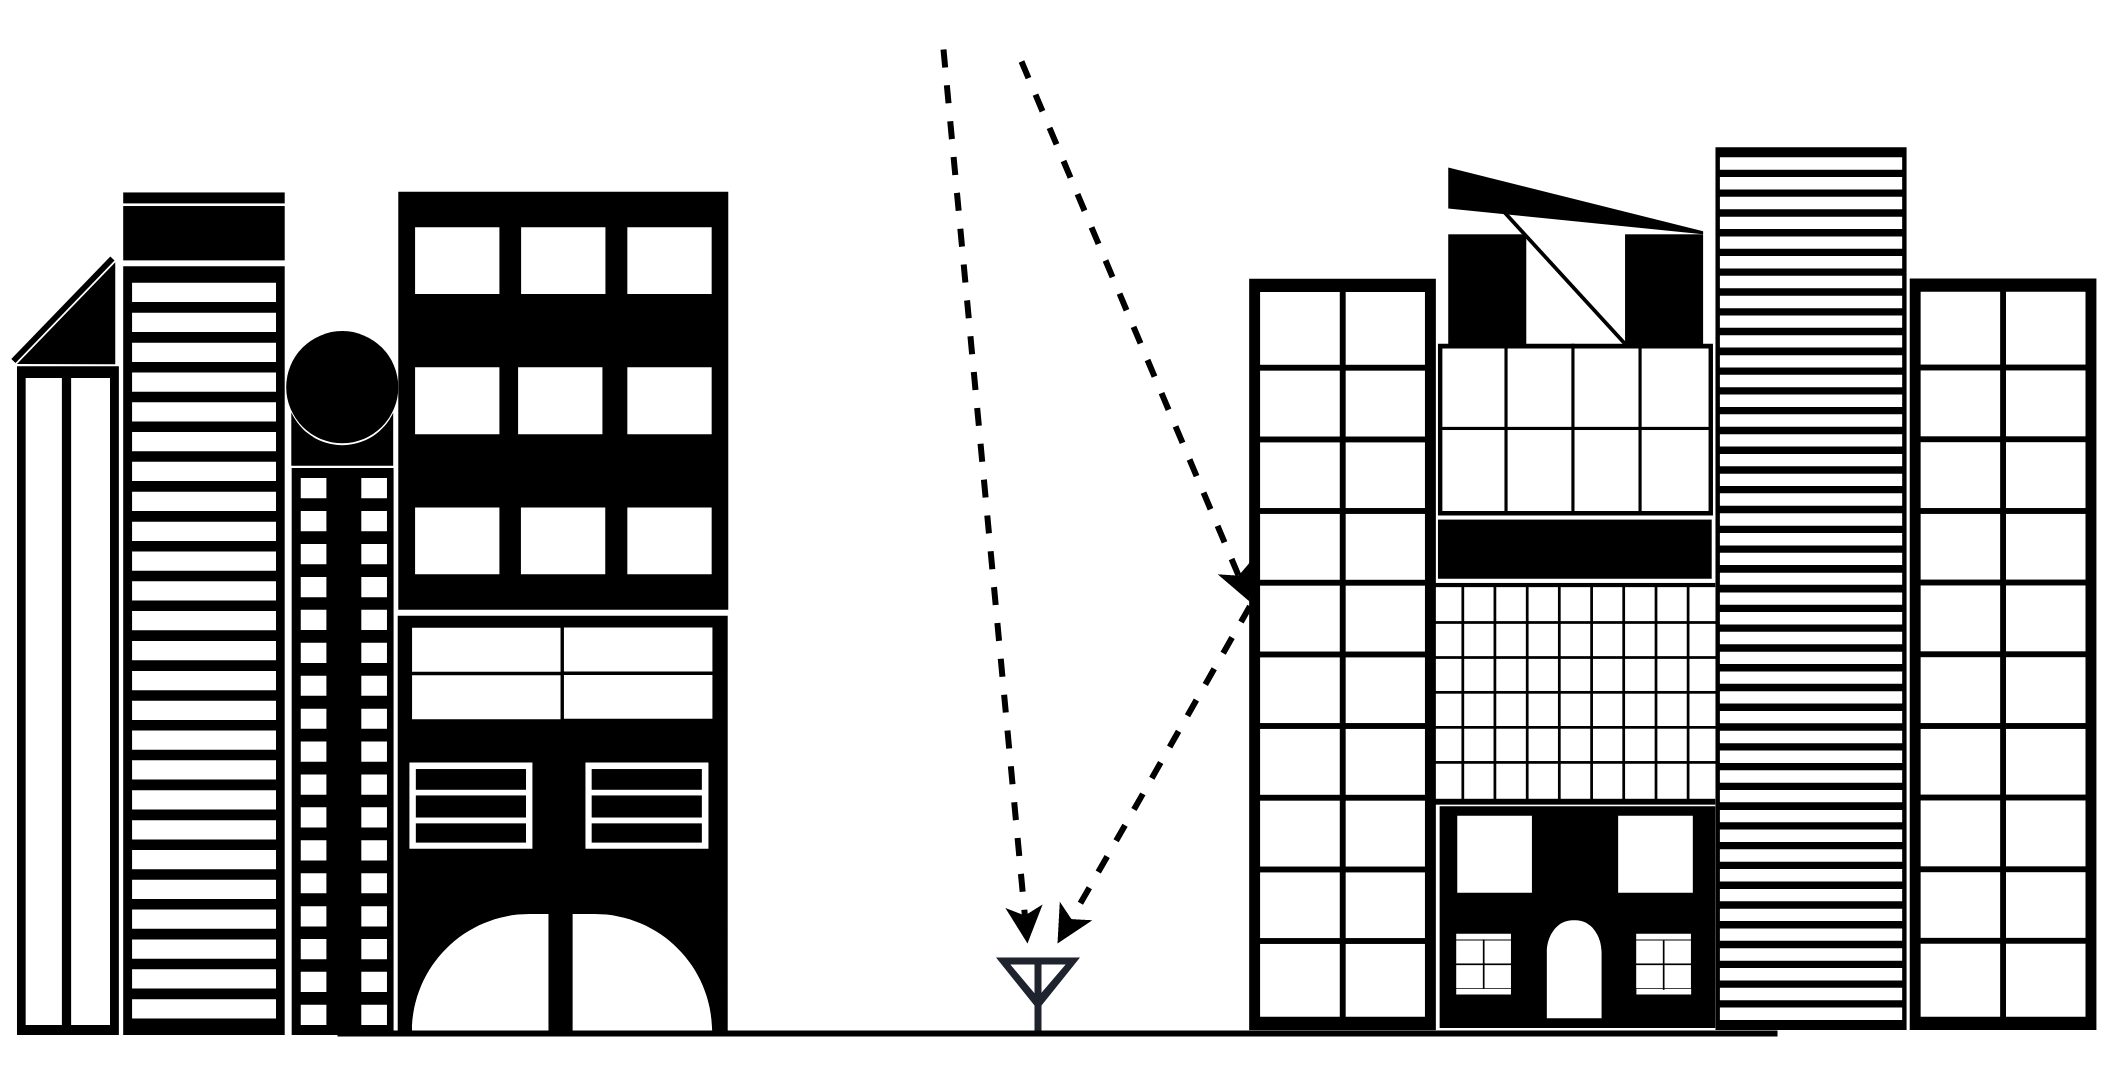
\includegraphics[width=\textwidth]{images/Multipath.png}
 \captionof{figure}{Multipath in an urban canyon}
\end{minipage}
\hfill
\begin{minipage}{0.45\textwidth}
 \flushright
 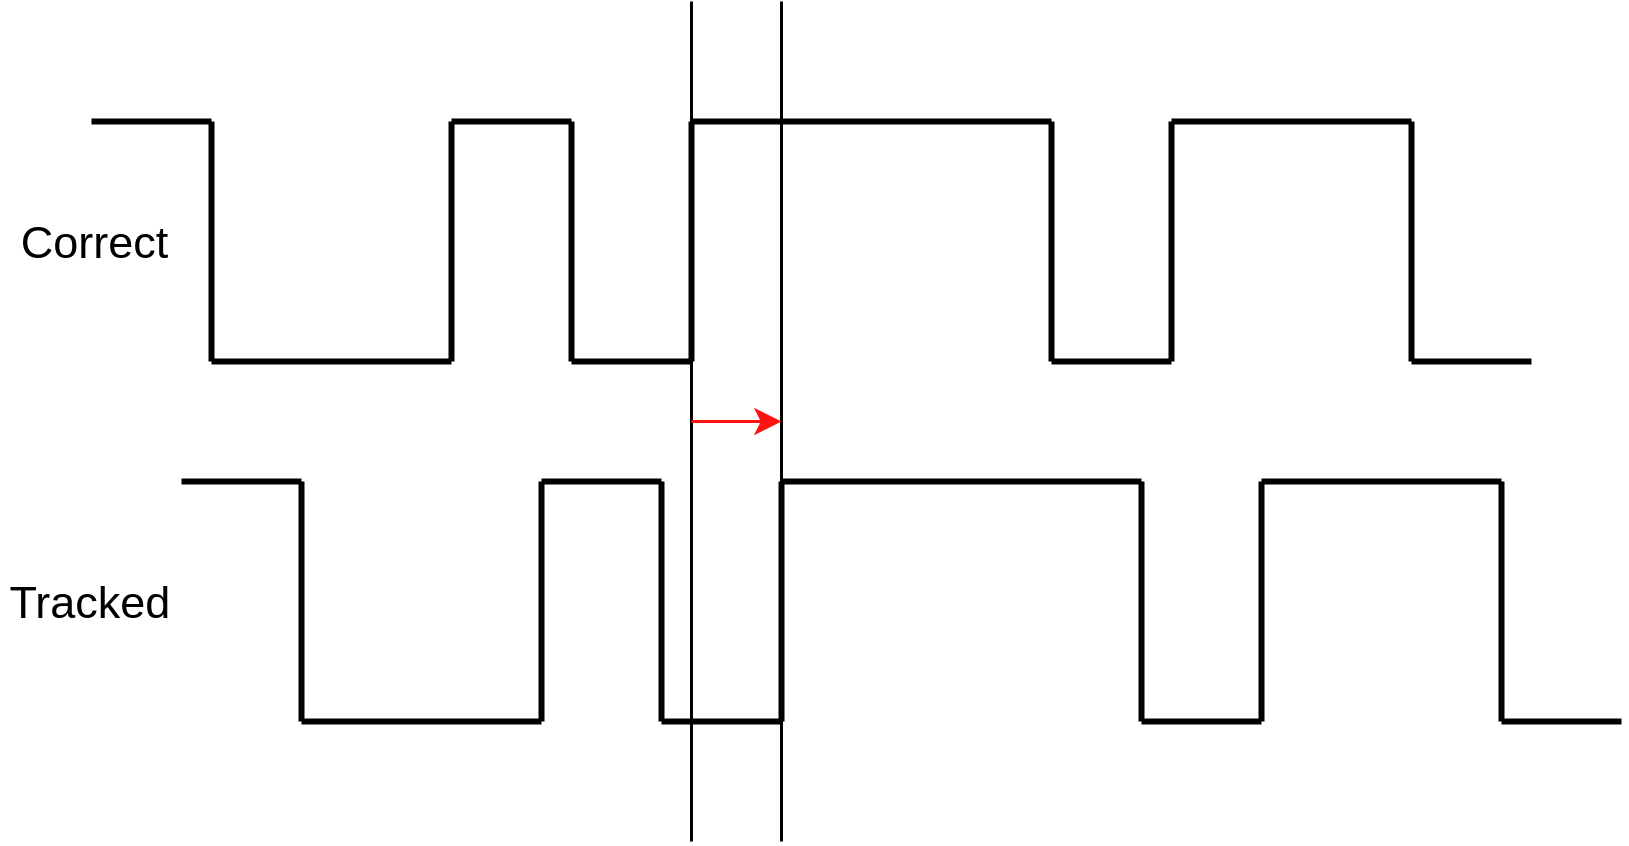
\includegraphics[width=\textwidth]{images/Receiver_Noise.png}
 \captionof{figure}{Tracking error caused by receiver noise}
\end{minipage}

